% !TeX encoding = UTF-8
% !TeX spellcheck = hu_HU

\chapter{A Qt és GTK keretrendszerek áttekintése}\label{sect:qtgtkoverview}


\section{Bemutatás, rövid történet}
A GTK és a Qt (ejtése mint az angol \textit{cute} szó) széles körben elterjedt GUI eszközkészlet-keretrendszerek. Mindkettővel lehetőség van összetett felhasználói felületek készítésére, a Qt által biztosított osztályok ezen kívül lehetőséget adnak komplex alkalmazások létrehozására is.

A Qt és a GTK története is az 1990-es évekre vezethető vissza. A Qt fejlesztését 1990~nyarán kezdte meg Haavard Nord és Eirik Chambe-Eng, amikor egy ultrahangfelvételek tárolására alkalmas programot fejlesztettek \cite{QtWiki}. Később céget alapítottak, 1994-ben megalakult a Quasar Technologies, ami később Trolltech-ként vált ismertté, manapság pedig a The~Qt~Company nevet viseli. A keretrendszer köré szerveződött cég jól mutatta, hogy a Qt alkotói pénzt szerettek volna keresni a könyvtárral, így a licence nem engedte a szabad terjesztést. Ez először akkor kezdett problémává válni, amikor a KDE -- egy népszerű Linux asztali környezet -- bebiztosította a helyét a túlnyomórészt szabad szoftverekből álló Linuxos világban.

\begin{figure}[h]
	\centering
	\begin{subfigure}{0.4\textwidth}
		\centering
		
\includegraphics[keepaspectratio, scale=0.18]{figures/qt-logo}
	\end{subfigure}
	\hspace{0.075\textwidth}
	\begin{subfigure}{0.3\textwidth}
		\centering
		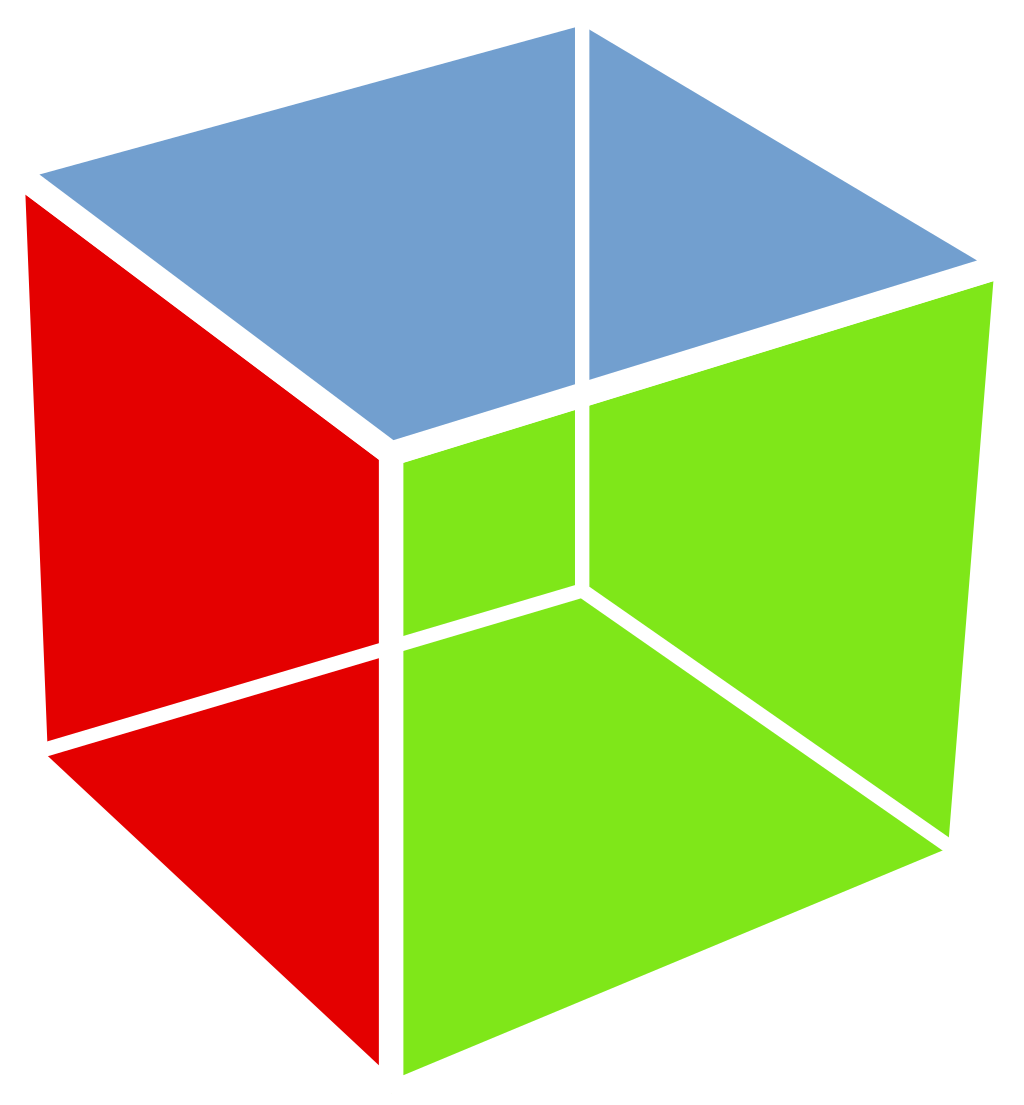
\includegraphics[keepaspectratio, scale=0.11]{figures/gtk-logo}
	\end{subfigure}
	\caption{A Qt és a GTK logója}
	\label{fig:qtgtklogo}
\end{figure}

A GTK történetének kezdete körülbelül 1996-ra tehető, ekkor kezdte meg ugyanis Peter Mattis a keretrendszer fejlesztését \cite{GtkWiki}. A cél a GIMP-hez akkor használt Motif GUI eszközkészlet lecserélése volt (a könyvtár eredeti neve, a GIMP ToolKit is innen ered), amit végül az 1998~nyarán megjelent 1.0-s GIMP verzióval sikerült is véghez vinni.

Mindkét technológia elterjedésében jelentős szerepe volt annak, hogy a '90-es évek végén nagyobb asztali környezetek kezdték el használni mind a Qt, mind a GTK könyvtárakat. A KDE-projekt a Qt egyik legjelentősebb felhasználója és számos változtatással segítik a keretrendszer fejlődését, míg a GNOME asztali környezet fejlesztése a GTK alakulására van nagy hatással. Fontos különbség azonban a fent már említett licencelés problémája: a Qt egy kereskedelmi forgalomban lévő szoftvercsomag, mely néhány kisebb kivétellel (pl. nyílt forráskódú projektek \cite{QtOpenSource}, oktatási célok \cite{QtEdu}) csak licencdíj megfizetése ellenében használható. Ez sokaknak nem tetszett a szabad szoftverekben bővelkedő Unixos világban, így ez is motiválta a GTK korai fázisában a fejlesztést, ugyanis a GTK teljesen szabad licenccel rendelkezik, bárki szabadon felhasználhatja, módosíthatja és terjesztheti is.

\section{Technológiai áttekintés}
% qt xml, qml json, gtk
% gtk builder, qt creator, qt .ui
A Qt elsődleges programozási nyelve a C++, míg a GTK-é a C, bár mindkettőhöz léteznek megoldások más nyelvekkel való együttműködés biztosítására is, mint például Python és C++.

A felhasználói felületek leírásához alapvetően mindkét technológia XML-alapú megoldást használ, bár a Qt esetében lehetőség van a JSON-alapú QML használatára is. A~QML~(Qt~Modeling~Language) egy deklaratív felhasználóifelület-leíró nyelv, melyet a Nokia fejlesztett a Qt projekthez 2009 környékén \cite{QmlWiki}. Előnye az XML-alapú megoldáshoz képest, hogy könnyebben áttekinthető, valamint lehetőséget biztosít JavaScript használatára is, így például a KDE számos alkalmazását folyamatosan portolják -- azaz a funkcionalitás megtartása mellett, általában a felhasználók számára láthatatlan módon megváltoztatják a használt könyvtárakat és a kódbázist -- át a hagyományos C++ és XML technológia helyett a QML-esre (ugyanakkor a QML részei is elérhetőek C++ kódból, például lehetőség van eseménykezelők regisztrálására is).

% TODO: gtk builder vs qt xml-es gui felépítése
% qt a .ui fájlokból a uic segítségével generál ui osztályokat
% gui editorok
A felületleírókban megadott kinézet előállításához a GTK a GTK Builder\footnote{\url{https://docs.gtk.org/gtk3/class.Builder.html}} osztályt használja, míg a Qt a \texttt{uic} segédprogram segítségével generál osztályokat a \texttt{.ui} fájlokból~\cite{qtnotepadtutorial}. Az így generált osztályok a \texttt{Ui} névtéren belül érhetőek el. A felület kódbeli inicializálását az alábbi táblázat mutatja be:
\begin{table}[h]
	\centering
	\begin{tabular}{|c|c|}
		\hline
		Qt & GTK \\
		\hline
		\begin{minipage}{0.35\linewidth}
			\begin{lstlisting}
ui(new Ui::Notepad);
ui->setupUi(this);
			\end{lstlisting}
		\end{minipage}
		&
		\begin{minipage}{0.35\linewidth}
			\begin{lstlisting}
Gtk::Builder::
    new_from_file("ui.glade")
			\end{lstlisting}
		\end{minipage} \\
		\hline
	\end{tabular}
	\label{tab:qtgtkxmlbuild}
	\caption{XML-ben definiált felhasználói felület inicializálása Qt-t és GTK-t használó programokban}
\end{table}

Mivel mindkét szóban forgó keretrendszer lehetőséget biztosít összetett felhasználói felületek létrehozására, és ezek leírása kézzel nagyon körülményes lenne, ezért lehetőség van a felhasználói felületek vizuális összeállítására. Mind a Qt, mind a GTK rendelkezik ilyen programmal: Qt esetében ilyen például a Qt Creator, míg GTK-nál a Glade a legnépszerűbb GUI összeállító program. Bár a \textit{Design} nézet mindkét szerkesztő esetén ugyanazt a célt szolgálja, a két alkalmazás jelentősen eltér egymástól: a Qt Creator egy fejlesztői környezet, mely rendelkezik \textit{Design} nézettel (de emellett lehetőség van pl. C++ forráskód írására, valamint a projekt buildelésére is), a Glade viszont kizárólag a felület összeállításában játszik szerepet. A későbbiekben az ilyen programokkal létrehozott UI-leírók feldolgozására összpontosítunk.

{
\kep[0.35]{figures/qtcreator.png}{A Qt Creator felhasználói felülete design nézetben}{qtcreator}
\kep[0.402]{figures/glade.png}{A Glade felhasználói felülete}{glade}}

\begin{landscape}
	\thispagestyle{empty} % oldalszámozás kihagyása a fektetett oldalon
	\centering % táblázat középre igazítása
	\begin{table}
	\begin{tabular}{|c|c|c|}
		\hline
		QML & Qt XML & GTK XML \\
		\hline
		\begin{minipage}[t]{0.3\linewidth}
			\begin{lstlisting}[numbers=left, xleftmargin=8mm]
QWidget {
    name: "centralWidget"
    QPushButton {
        name: "pushButton"
        geometry: {
            x: 10
            y: 20
            width: 150
            height: 50
        }
        text: "Hello World!"
    }
}
			\end{lstlisting}
		\end{minipage}
		&
		\begin{minipage}[t]{0.3\linewidth}
			\begin{lstlisting}[language=xml, numbers=left, xleftmargin=8mm]
<widget class="QWidget"
	    name="centralWidget">
  <widget class="QPushButton"
          name="pushButton">
    <property name="geometry">
      <rect>
        <x>10</x>
        <y>20</y>
        <width>150</width>
        <height>50</height>
      </rect>
    </property>
    <property name="text">
      <string>Hello World!</string>
    </property>
  </widget>
</widget>
			\end{lstlisting}
		\end{minipage}
		&
		\begin{minipage}[t]{0.3\linewidth}
			\begin{lstlisting}[language=xml, numbers=left, xleftmargin=8mm]
<object class="GtkFrame">
  <child>
    <object class="GtkButton"
        id="pushButton">
      <property name="label"
          translatable="yes">
          Hello World!
        </property>
        <property name="name">
          pushButton
        </property>
    </object>
  </child>
</object>
			\end{lstlisting}
		\end{minipage} \\
		\hline
	\end{tabular}
	\caption{A QML, Qt XML és a GTK XML felépítésének összehasonlítása}
	\label{tab:sourcecomparison}
	\end{table}
\end{landscape}
